\documentclass[10pt]{IEEEtran}
\usepackage[backend=biber,style=phys]{biblatex}
\usepackage{amsmath}
\usepackage{amsfonts}
\usepackage{amssymb}
\usepackage{caption}
\usepackage{graphicx}
\usepackage{hyperref}
\usepackage{hhline}
\usepackage{listings}
\usepackage{multirow}
\usepackage{subcaption}
\lstset{language=C++}
\usepackage{csquotes}
\usepackage{url}
\graphicspath{{./images/}}
\addbibresource{rutherford.bib}

\begin{document}

% Define document title and author
    \title{Rutherford Scattering}
    \author{Jamison Lahman, Brandon Coleman, Kenny Richely, Joe Pincura, Jacob Williamson, and Taylor Grueser
    \thanks{Instructor: Paul King}}
    \maketitle

% Write abstract here
\begin{abstract}
Projecting charged alpha particles at a target sample can be used to estimate the charge and cross-sectional area the target element's nuclei. Through the Coulomb potential, the incoming alpha particles can be deflected and scattered accordingly. Using spectroscopy to identify the resulting energy of the incident alpha particles, we were able to identify an elemental composition of the target. We experimentally determined a target composition of 81.53$\pm$0.17\% gold, 12.15$\pm$0.14\% silver, and 6.32$\pm$0.19\% copper which agrees with the theoretical values of 81\% gold, 12\% silver, and 7\% copper. Additionally, we experimentally determined cross-sectional areas which were consistent with the theoretical values when considering all sources of error.
\end{abstract}
\section{Introduction \& Theory}
When a charged particle approaches the nucleus of an atom, the Coulomb potential scatters the oncoming particle. The Coulomb potential is responsible for the static electric force that charged particles experience. The Coulomb potential is given by:
\begin{equation}
U(r) = \frac{Z_0Z_1 e^2}{4\pi\epsilon_0r},
\end{equation}
where $Z_0$ and $Z_1$ are the charges of the two particles and r is the separation\cite{blackboard}. Through elastic collisions, the charge and size of various nuclei can be determined. Alpha particles, doubly ionized helium atoms, are directed towards a material. The nucleus of the atoms of the material are much smaller than the atom themselves and of similar charge as the alpha particle which produces an opportunity for scattering, though it is a small chance. Luckily, many atoms are packed tightly together in  material making collisions common enough to observe.

The theoretical Rutherford cross-section is given by the following equation:
\begin{equation}
\frac{d\sigma}{d\Omega} = 1.296\left(\frac{Z_0 Z_1}{E_0}\right)^2\left[\frac{1}{\sin^4(\theta/2)}-2\left(\frac{M_0}{M_1}\right)^2\right],
\end{equation}
where $M_0$ and $M_1$ are the particles' respective masses, $E_0$ is the incident energy, and $\theta$ is the laboratory scattering angle. The Rutherford cross-section will be calculable experimentally by the equation\cite{blackboard},
\begin{equation}
\frac{d\sigma}{d\Omega} = \frac{N_{peak}/(1-dt)}{Nn\Delta\Omega},
\end{equation}
where $N_{peak}$ is the number of counts in a given peak, $dt$ is the fractional dead time, $N$ is the number of incident alpha particles, $n$ is the number of nuclei per cm$^2$ given by the equation,
\begin{equation}
n = \frac{6.54\times10^{17}}{\cos(\theta_{target})}\text{ atoms/cm$^2$}.
\end{equation}

The solid angle is dependent on the target angle, $\theta_{target}$, rather than the scattering angle. The solid angle is given by the equation,

Because the likelihood of an alpha particle depends on both the number of elemental nuclei as well as the size, the number of counts at each energy position are dependent on these factors. The peak for each element can be related to the other elemental peaks to determine the number of nuclei for each element through the relation,
\begin{equation}
\frac{N_{peak,0}}{N_{peak,1}} = \frac{\sigma_{0}n_{0}}{\sigma_{1}n_{1}},
\end{equation}
and $\sigma$ is the cross-sectional area of the elemental nucleus given by equation (2).

The fractional composition difference between two elements is,
\begin{equation}
\frac{f_0}{f_1} =  \frac{n_0/n}{n_1/n} = \frac{n_0}{n_1}.
\end{equation}
The fractional composition for a given element is therefore,
\begin{equation}
f_i = \frac{n_i}{n_{total}} = \frac{f_i}{\Sigma f} = \frac{1}{1+\Sigma (f_n/f_i)}
\end{equation}
with $f_n$ being the fractional composition of element $n$.


\begin{figure}
       \begin{center}
       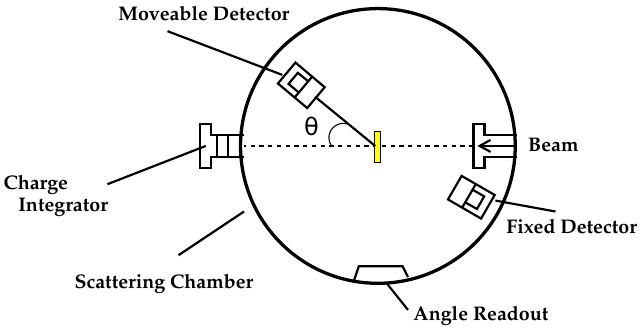
\includegraphics[width=\columnwidth]{setup.png}
       \caption{A simplified schematic of the setup apparatus. The gold foil target is placed at the center of the chamber while two detectors are placed radially around the target. The angles are observed through the angle readout\cite{blackboard}.}
       \label{fig:setup}
       \end{center}
\end{figure}

\begin{figure}
       \begin{center}
       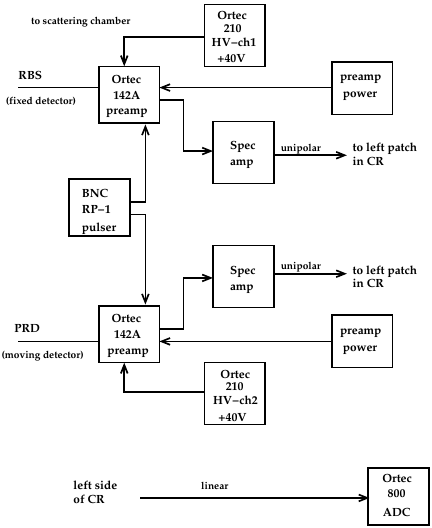
\includegraphics[width=\columnwidth]{depth.png}
       \caption{The total paths from alpha source to detectors then to all necessary amplification before processing using DAQ software\cite{blackboard}.}
       \label{fig:depth}
       \end{center}
\end{figure}

\section{Experimental Details}
All of the data was collected using Edwards Accelerator Laboratory at Ohio University in Athens, Ohio. Situated at the center of the chamber, shown in Fig. \ref{fig:setup}, was a target of non-pure gold foil with a composition of approximately 81\% gold, 12\% silver, and 7\% copper. In total, the lab apparatus consisted of two solid-state silicon detectors. A more in-depth experimental design for each detector is given by Fig. \ref{fig:depth}. The data was collected using DAQ software.

After inspecting the chamber for defects, we measured the dimensions of the apparatus. The aperture of the movable detector was 3.59mm and was 78.00mm from the target. The fixed detector had an aperture of 3.67 and was 63.00mm from the target. In total, we performed 12 experiential runs.

The experiment has four sources of error. In addition to the random error on our peaks, $\epsilon_N$, there is additionally an error on $n$ and the observational error in out angle measurements. The relative errors of the peak counts are both approximately 1\% while the error on the angle measurements is estimated to be a few percent. The largest source of error is likely to be on $n$ which is set at 10\%. Despite being lower relative errors, the errors on the peaks are the only source of point-to-point errors. $\epsilon_n$ and $\epsilon_{\Delta\Omega}$ are both constant throughout the experiment. The total error on $\sigma$ is given by: 

\begin{equation}
\frac{\epsilon_\sigma}{\sigma} = \sqrt{\left(\frac{\epsilon_{N_{peak}}}{N_{peak}}\right)^2+\left(\frac{\epsilon_{N}}{N}\right)^2+\left(\frac{\epsilon_{n}}{n}\right)^2+\left(\frac{\epsilon_{\Delta\Omega}}{\Delta\Omega}\right)^2}
\end{equation}

\section{Data}    

Unfortunately, the accelerator we were using was experiencing technical problems resulting in a lack of high-energy runs. We managed to collect data for one run with 5 MeV alphas. The spectra are plotted in Fig. \ref{fig:5RBS} and \ref{fig:5PRD} while peak analysis is performed in Tab. \ref{tab:5RBS} and \ref{tab:5PRD}.

\begin{figure}[!hbt]
       \begin{center}
       5 MeV Run Using RBS Detector
       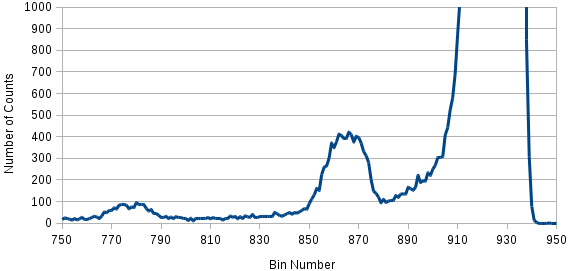
\includegraphics[width=\columnwidth]{5mevrbs}
       \caption{The spectrum produced by the RBS detector for 5 MeV alpha particles. From left to right, the peaks indicate copper, silver, and gold particles in the target. Scattering due to gold occurred roughly 200 times as often as silver. Much of the gold peak was omitted to show details of the other peaks.}
       \label{fig:5RBS}
       \end{center}
\end{figure}

     \begin{table}[!hbt]
        % Center the table
        \begin{center}
        % Title of the table
        \caption{5 MeV Run Using RBS Detector}
        \label{tab:5RBS}
        \begin{tabular}{c|ccccccc}
             Element & $N$ & $\sigma_N$ & $\bar{x}$ & $\sigma_{\bar{x}}$ & RMS & $f$ & $\sigma_f$\\
             \hline\hline
			Au & 159388 & 399.23 & 924.99 & 0.02 & 7.07 & 81.53 & 0.17 \\
			Ag & 8393 & 91.61 & 864.85 & 0.08 & 6.95 & 12.15 & 0.14 \\
			Cu & 1654 & 40.67 & 777.61 & 0.16 & 6.44 & 6.32 & 0.19 \\
			\hline
        \end{tabular}\\
        \end{center}
                Peak analysis of the 5 MeV run using the RBS detector. The concentration of and type of element present in the target are indicated by the position and strength of the peaks. Using the number of peaks along with the theoretical cross-sections, we found fractional compositions for each element following Eq. (7). We determine the target to be $81.53\pm0.17\%$ gold, $12.15\pm0.14\%$ silver, and $6.32\pm0.19\%$ copper.
    \end{table}
    
\begin{figure}[!hbt]
       \begin{center}
       5 MeV Run Using PRD Detector
       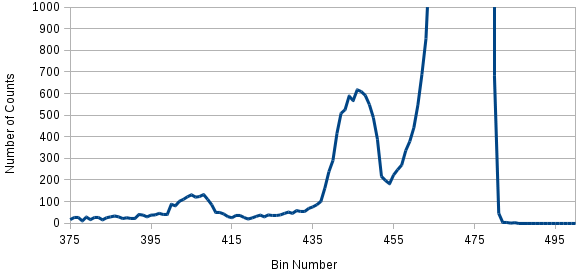
\includegraphics[width=\columnwidth]{5mevprd}
       \caption{The spectrum produced by the PRD detector for 5 MeV alpha particles. From left to right, the peaks indicate copper, silver, and gold particles in the target. Scattering due to gold was dominate so the peak was truncated to show details of the other peaks.}
       \label{fig:5PRD}
       \end{center}
\end{figure}    
    
    \begin{table}[!hbt]
        % Center the table
        \begin{center}
        % Title of the table
        \caption{5 MeV Runs Using PRD Detector}
        \label{tab:5PRD}
        \begin{tabular}{c|ccccccc}
             Element & $N$ & $\sigma_N$ & $\bar{x}$ & $\sigma_{\bar{x}}$ & RMS & $f$ & $\sigma_f$\\
             \hline\hline
			Au & 12789 & 472.73 & 472.73 & 0.01 & 3.75 & 80.37 & 0.19 \\
			Ag & 7391 & 85.97 & 445.56 & 0.05 & 4.31 & 13.14 & 0.16 \\
			Cu & 1384 & 37.20 & 405.71 & 0.10 & 3.64 & 6.49 & 0.21 \\
			\hline
        \end{tabular}\\
        \end{center}
                Peak analysis of the 5 MeV run using the RBS detector. The concentration of and type of element present in the target are indicated by the position and strength of the peaks. Using the number of peaks along with the theoretical cross-sections, we found fractional compositions for each element following Eq. (7). We determine the target to be $80.37\pm0.19\%$ gold, $13.14\pm0.16\%$ silver, and $6.49\pm0.21\%$ copper.
    \end{table}


\begin{figure*}[!hbt]
	\begin{center}
    \begin{subfigure}[!hbt]{0.49\textwidth}
    	   \centering{Low Energy Runs Using RBS Detector} \\
        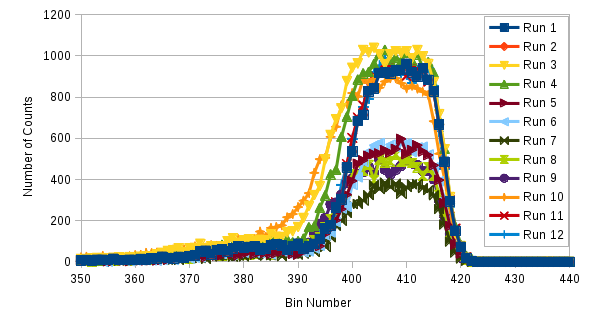
\includegraphics[width=\textwidth]{lowrbs.png}
        \caption{The number of counts and shape of the peaks in the RBS detector are both fairly uniform across runs. This implies there is not a large dependency on the detector angle.}
        \label{fig:lowrbs}
    \end{subfigure}\hfill
    ~ %add desired spacing between images, e. g. ~, \quad, \qquad, \hfill etc. 
    %(or a blank line to force the subfigure onto a new line)
    \begin{subfigure}[!hbt]{0.49\textwidth}
    		\centering{Low Energy Runs Using PRD Detector}
        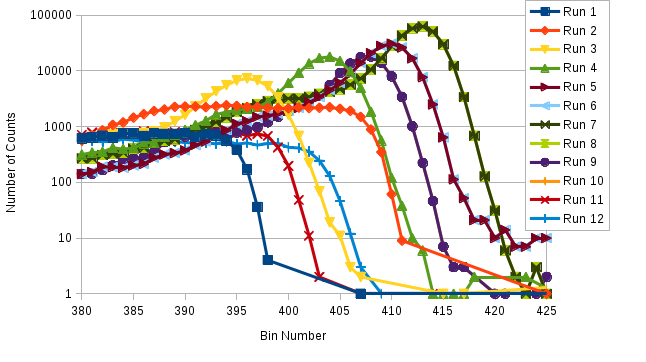
\includegraphics[width=\textwidth]{loglowprd.png}
        \caption{The number of counts and location of the peak in the PRD detector for runs with varying detector angles. The number of counts drastically changes by orders of magnitude suggestion a large angle dependency.}
        \label{fig:lowprd}
    \end{subfigure}
    \caption{Low energy runs at various detector angles. As expected, the counts in Fig. 5(a) show the RBS detector is roughly independent of the angle while the counts in Fig. 5(b) shows the PRD has a large angle dependency.}
    \label{fig:lowenergy}
    \end{center}
\end{figure*}

\begin{table*}[!hbt]
        % Center the table
        \begin{center}
        % Title of the table
        \caption{Constant Values for Both Detectors in Low Energy Runs}
        \label{tab:lowconst}
        \begin{tabular}{|c|cccccccccccc|}
            \hline
		   Run & 1 & 2 & 3 & 4 & 5 & 6 & 7 & 8 & 9 & 10 & 11 & 12 \\ 
            \hline\hline
            $N_0$ (E+12) & 3.13 & 3.13 & 3.13 & 3.13 & 1.69 & 1.56 & 1.13 & 1.56 & 1.60 & 3.13 & 3.13 & 3.13 \\
		   \hline            
            $\epsilon_{N_{0}}$ (E+09) & 3.13 & 3.13 & 3.13 & 3.13 & 3.13 & 3.13 & 3.13 & 3.13 & 3.13 & 3.13 & 3.13 & 3.13 \\ 
            \hline
            $\theta_{target}$ (rad)& 0.00 & 5.50 & 0.79 & 0.61 & 0.44 & 0.35 & 5.93 & 5.89 & 5.76 & 5.59 & 0.00 & 0.00 \\
            \hline
            $\theta_{detector}$ (rad)& 2.44 & 1.57 & 1.57 & 1.22 & 0.87 & 0.70 & 5.59 & 5.50 & 5.24 & 4.89 & 4.19 & 4.54 \\
            \hline
            $n$  (E+17/cm$^2$) & 6.54 & 9.25 & 9.25 & 7.98 & 7.22 & 6.96 & 6.96 & 7.08 & 7.55 & 8.54 & 6.54 & 6.54 \\
            \hline
            $\epsilon_n$  (E+16/cm$^2$) & 6.54 & 9.25 & 9.25 & 7.98 & 7.22 & 6.96 & 6.96 & 7.08 & 7.55 & 8.54 & 6.54 & 6.54 \\
            \hline
        \end{tabular}
        \end{center}
    \end{table*}
    
    \begin{table*}[!hbt]
        % Center the table
        \begin{center}
        % Title of the table
        \caption{Low Energy Runs Using RBS Detector}
        \label{tab:lowRBS}
        \begin{tabular}{|c|cccccccccccc|}
            \hline
		   Run & 1 & 2 & 3 & 4 & 5 & 6 & 7 & 8 & 9 & 10 & 11 & 12 \\ 
		   \hline      \hline      
            $N$ & 18844 & 24633 & 25543 & 22987 & 11857 & 11857 & 8133 & 11069 & 11462 & 23471 & 19413 & 19210 \\
		   \hline  
            $\sigma_N$ & 137 & 157 & 160 & 152 & 109 & 109 & 90 & 105 & 107 & 153 & 139 & 139 \\
            \hline
            $\bar{x}$ & 404.36 & 398.60 & 401.42 & 402.63 & 403.37 & 403.57 & 402.32 & 402.37 & 401.39 & 399.86 & 403.77 & 403.81 \\
            \hline
            $\sigma_{\bar{x}}$ & 0.09 & 0.10 & 0.09 & 0.09 & 0.13 &  0.13 & 0.17 & 0.14 & 0.14 & 0.10 & 0.10 & 010 \\
		   \hline            
            $dt$ (\%) & 1.15 & 1.41 & 1.49 & 1.38 & 0.65 & 0.18 & 0.16 & 0.64 & 0.63 & 1.33 & 1.00 & 1.01 \\
            \hline
		   $\Delta\Omega$ (E-03 sr) & 2.69 & 2.69 & 2.69 & 2.69 & 2.69 & 2.69 & 2.69 & 2.69 & 2.69 & 2.69 & 2.69 & 2.69 \\
		   \hline
		   $\epsilon_{\Delta\Omega}$ (E-05 sr) & 5.18 & 5.18 & 5.18 & 5.18 & 5.18 & 5.18 & 5.18 & 5.18 & 5.18 & 5.18 & 5.18 & 5.18 \\
		   \hline
		   $\sigma$ (E-24 cm$^2$) & 3.46 & 3.21 & 3.33 & 3.47 & 3.64 & 4.05 & 3.84 & 3.74 & 3.54 & 3.31 & 3.56 & 3.52 \\
		   \hline
		   PW Error (E-25 cm$^2$) & 0.37 & 0.54 & 0.55 & 0.96 & 3.2 & 7.0 & 10 & 5.2 & 2.1 & 0.72 & 0.44 & 0.53 \\
		   \hline
		   Total Error (E-24 cm$^2$) & 0.46 & 1.3 & 1.3 & 3.2 & 1.1 & 28 & 32 & 19 & 6.1 & 2.1 & 0.64 & 9.2 \\
		   \hline
		   Residual (E-24 cm$^2$) & 2.41 & 1.69 & 1.25 & 2.64 & 3.95 & 7.57 & 5.27 & 4.87 & 2.82 & 8.63 & 3.24 & 2.85 \\
		   \hline
		   \% Error & 7.61 & 0.54 & 3.95 & 8.35 & 12.50 & 23.93 & 16.66 & 15.40 & 8.92 & 2.73 & 9.91 & 8.99 \\
		   \hline
        \end{tabular}
        \end{center}
        Data from the low energy runs using the RBS. Dead time is the dead time right. The residuals are calculated using the theoretical value from Eq. (2) which were $\sigma_{au} = 3.67\times10^{-24}$cm$^2$, $\sigma_{ag} = 1.30\times10^{-24}$cm$^2$, and $\sigma_{au} = 4.91\times10^{-25}$cm$^2$.  Multiplying the cross-sections by the theoretical, relative abundances in the target, the total cross-section is estimated to be $\sigma = 3.16\times10^{-24}$cm$^2$.
    \end{table*}    
    
    
    \begin{table*}[!hbt]
        % Center the table
        \begin{center}
        % Title of the table
        \caption{Low Energy Runs Using PRD Detector}
        \label{tab:lowPRD}
        \begin{tabular}{|c|cccccccccccc|}
            \hline
		   Run & 1 & 2 & 3 & 4 & 5 & 6 & 7 & 8 & 9 & 10 & 11 & 12 \\ 
		   \hline       \hline     
            $N$ & 15292 & 59688 & 61340 & 122839 & 190580 & 455843 & 378242 & 290580 & 11350 & 86462 & 21230 & 30273 \\
		   \hline  
            $\sigma_N$ & 124 & 244 & 248 & 350 & 437 & 675 & 615 & 544 & 337 & 294 & 146 & 174 \\
            \hline
            $\bar{x}$ & 383.07 & 392.50 & 392.18 & 400.92 & 407.61 & 409.44 & 409.91 & 409.22 & 405.16 & 397.87 & 384.30 & 370.68 \\
            \hline
            $\sigma_{\bar{x}}$ & 0.07 & 0.05 & 0.03 & 0.02 & 0.01 &  0.01 & 0.01 & 0.01 & 0.02 & 0.02 & 0.07 & 012 \\
		   \hline
            $dt$ (\%) & 0.92 & 3.80 & 3.40 & 7.02 & 13.48 & 10.65 & 7.65 & 15.43 & 6.15 & 4.59 & 1.20 & 2.22 \\
			\hline            
			$\Delta\Omega$ (E-03 sr) & 1.66 & 1.66 & 1.66 & 1.66 & 1.66 & 1.66 & 1.66 & 1.66 & 1.66 & 1.66 & 1.66 & 1.66 \\
			\hline
			$\epsilon_{\Delta\Omega}$ (E-05 sr) & 2.3 & 2.3 & 2.3 & 2.3 & 2.3 & 2.3 & 2.3 & 2.3 & 2.3 & 2.3 & 2.3 & 2.3\\
			\hline
			$\sigma $ (E-24 cm$^2$)& 4.54 & 12.9 & 13.2 & 31.8 & 109 & 282 & 313 & 190 & 6.02 & 20.4 & 36.32 & 9.11 \\
			\hline
			PW Error (E-26 cm$^2$) & 3.7 & 5.4 & 5.5 & 9.6 & 32 & 70 & 100 & 52 & 21 & 7.2 & 4.4 & 5.3 \\
			\hline
			Total Error (E-24 cm$^2$)& 0.46 & 1.3 & 1.3 & 3.2 & 1.1 & 28 & 32 & 19 & 6.1 & 2.1 & 6.4 & 9.2 \\
		    \hline
		    $\sigma_{theory}$ (E-24 cm$^2$) & 4.22 & 13.2 & 13.2 & 30.4 & 103 & 241 & 154 & 52.7 & 19.3 & 5.86 & 9.57 & 2.85 \\
		    \hline
		    Residual (E-24 cm$^2$) & -0.32 & -0.27 & -0.03 & -1.39 & -103 & -241 & -241 & -154 & -52.7 & -19.3 & -5.86 & -9.57 \\
		    \hline 
		    \% Error & -7.48 & -2.08 & -0.21 & -4.55 & -5.26 & -17.10 & -29.85 & -23.71 & -14.11 & -5.79 & -7.93 & 4.81 \\
		    \hline
        \end{tabular}
        \end{center}
        Data from the low energy runs using the RBS. Dead time is the dead time left. The residuals are calculated using the theoretical value from Eq. (2).
    \end{table*}     

\section{Results}
\begin{figure*}[!hbt]
	\begin{center}
    \begin{subfigure}[!hbt]{0.49\textwidth}
       \centering{RBS Cross-Section as a Function of Detector Angle} \\
       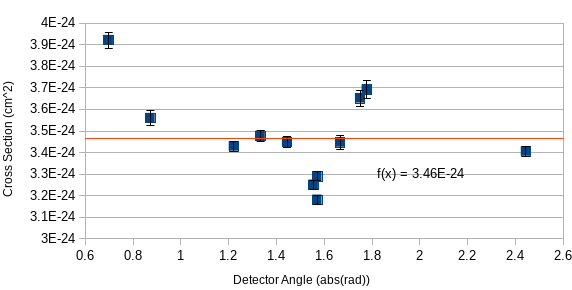
\includegraphics[width=\textwidth]{lowrbsres}
       \caption{As we expected, the theoretical cross-section is constant for all back scattering.}
       \label{fig:rbsres}
    \end{subfigure}\hfill
    ~ %add desired spacing between images, e. g. ~, \quad, \qquad, \hfill etc. 
    %(or a blank line to force the subfigure onto a new line)
    \begin{subfigure}[!hbt]{0.49\textwidth}
    	   \centering{PRD Cross-Section as a Function of Detector Angle} \\
       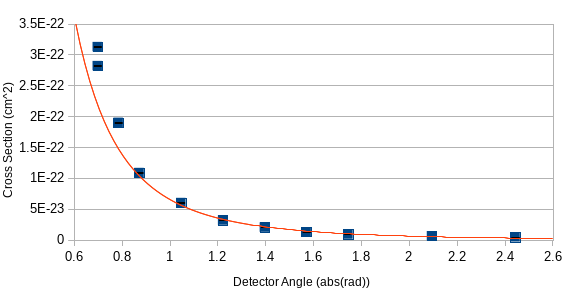
\includegraphics[width=\textwidth]{lowprdres}
       \caption{As we expected, the theoretical cross-section is highly dependent on the detector angle.}
       \label{fig:prdres}
    \end{subfigure}
    \caption{The red curve indicates the theoretical cross-section given by the Eq. 2. The points were determined using Eq. 3.}
    \label{fig:lowenergy}
    \end{center}
\end{figure*}

Out estimated composition of $81.53\pm0.17\%$ gold, $12.15\pm0.14\%$ silver, and $6.32\pm0.19\%$ copper from the RBS and $80.37\pm0.19\%$ gold, $13.14\pm0.16\%$ silver, and $6.49\pm0.21\%$ copper from the PRD agree nicely with the hypothesized composition of approximately 81\% gold, 12\% silver, and 7\% copper.

For the low energy runs, our observed data was in agreement theoretical values when all sources of error were taken into account. Considering only point wise error, as seen in Fig. \ref{fig:rbsres} and \ref{fig:prdres}, the agreement is lost, particularly in regards to the RBS data. Nevertheless, the cross-section in the PRD has an obvious detector angle dependency.
\section{Conclusion}

We experimentally determined a target composition of 81.53$\pm$0.17\% gold, 12.15$\pm$0.14\% silver, and 6.32$\pm$0.19\% copper as well as $80.37\pm0.19\%$ gold, $13.14\pm0.16\%$ silver, and $6.49\pm0.21\%$ copper, both of which agree with the theoretical values of 81\% gold, 12\% silver, and 7\% copper. Additionally, we experimentally determined cross-sectional areas which were consistent with the theoretical values, however when only considering the piece wise errors, this agreement vanishes. Because of this, we are confident concluding that, through elastic collisions, the charge and size of various nuclei can be experimentally determined.

\section{Acknowledgments}
I would like to thank my lab partners: Brandon Coleman, Kenny Richely, Joe Pincura, Jacob Williamson, and Taylor Grueser who helped with the setup, data acquisition and analysis for this report.
\printbibliography

\end{document}

% This is how you include a eps figure in your document. LaTeX only accepts EPS or TIFF files.
%    \begin{figure}[!hbt]
        % Center the figure.
%        \begin{center}
        % Include the eps file, scale it such that it's width equals the column width. You can also put width=8cm for example...
%        \includegraphics[width=\columnwidth]{}
        % Create a subtitle for the figure.
%       \caption{Simulation results on the AWGN channel. Average throughput $k/n$ vs $E_s/N_0$.}
        % Define the label of the figure. It's good to use 'fig:title', so you know that the label belongs to a figure.
%        \label{fig:tf_plot}
%        \end{center}
%    \end{figure}

    % This is how you define a table: the [!hbt] means that LaTeX is forced (by the !) to place the table exactly here (by h), or if that doesnt work because of a pagebreak or so, it tries to place the table to the bottom of the page (by b) or the top (by t).
%    \begin{table}[!hbt]
        % Center the table
%        \begin{center}
        % Title of the table
%        \caption{Simulation Parameters}
%        \label{tab:simParameters}
        % Table itself: here we have two columns which are centered and have lines to the left, right and in the middle: |c|c|
%        \begin{tabular}{|c|c|}
            % To create a horizontal line, type \hline
%            \hline
            % To end a column type &
            % For a linebreak type \\
%            Information message length & $k=16000$ bit \\
%            \hline
%            Radio segment size & $b=160$ bit \\
%            \hline
%            Rate of component codes & $R_{cc}=1/3$\\
%            \hline
%            Polynomial of component encoders & $[1 , 33/37 , 25/37]_8$\\
%            \hline
%        \end{tabular}
%        \end{center}
%    \end{table}

% You can cite a book or paper by using \cite{reference}.

% You can reference tables and figure by using the \ref{label} command. Each table and figure needs to have a UNIQUE label.
%Figures and tables should be labeled and numbered, such as in Table~\ref{tab:simParameters} and Fig.~\ref{fig:tf_plot}.
